\subsection{Enfoque funcional}

    A la hora de abordar el análisis de las redes ferroviarias, hemos encontrado que, a grandes rasgos, existen dos estrategias muy diferenciadas: el enfoque funcional y el enfoque geográfico, cada un con sus fortalezas y debilidades. Ambos enfoques se asemejan a la antigua discusión de arquitecturas CISC (del inglés, Complex Instruction Set Computing) vs RISC (del inglés, Reduced Instruction Set Computing), donde el primero centraliza las decisiones en un único módulo y el segundo distribuye las decisiones en pequeños módulos de funciones acotadas.    

    En el enfoque funcional las decisiones se basan en la 'tabla de enclavamientos', que define cada ruta que puede ser solicitada por el operario. Históricamente, tanto los enclavamientos mecánicos como los electromecánicos se han definido mediante tablas de enclavamientos, las cuales luego pueden ser usadas para definir la logística de la red. Es por eso que el personal técnico está muy capacitado tanto en la lectura de la tabla como en su elaboración.
    
    Cada ruta es definida junto con los elementos ferroviarios que la condicionan y los estados que deben tener los mismos para que la ruta sea habilitada. Además, se explicita cada una de las rutas que entrarían en conflicto con la ruta en cuestión. A modo de ejemplo se presenta en la Figura \ref{fig:funcional_1} como se realiza la asignación de rutas en un cambio de vías.

    \begin{figure}[h]
        \centering
        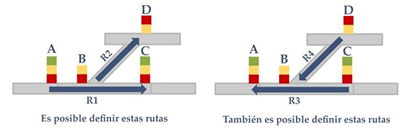
\includegraphics[width=1\textwidth]{Figuras/rutas.PNG}
        \centering\caption{Ejemplo de asignación de rutas.}
        \label{fig:funcional_1}
    \end{figure}

    Si el trazado de vías fuese utilizado para circular únicamente de izquierda a derecha, podemos definir únicamente dos rutas. La primera será la ruta R1, desde el semáforo A hasta el semáforo C. La segunda ruta R2 se define desde el semáforo B hasta el semáforo D, utilizando el cambio de vía a reverso. Ambas rutas quedan definidas en la Tabla \ref{Tab:funcional_2}.

    \begin{table}[!h]
        {
        \caption{Tabla de enclavamientos (rutas de izquierda a derecha).}
        \label{Tab:funcional_2}
        \centering
        %\small
            %\centering
            \begin{center}
            \resizebox{0.5\textwidth}{!}{
            \begin{tabular}{ c c c }
                \hline	
                   Ruta & Señal de entrada & Señal de salida \\	
                \hline
                   R$_1$ & Semáforo$_{\text{A}}$ & Semáforo$_{\text{C}}$ \\
                   R$_2$ & Semáforo$_{\text{B}}$ & Semáforo$_{\text{D}}$ \\
                %\hline
            \end{tabular}
            }
            \end{center}
        }    
    \end{table}
    
    De forma análoga, podríamos analizar el mismo trazado de vías asumiendo que las formaciones circularán estrictamente de derecha a izquierda, definiendo otro nuevo conjunto de rutas. Sumando así las rutas R3 y R4 como se visualiza en la Tabla \ref{Tab:funcional_3}

    \begin{table}[!h]
        {
        \caption{Tabla de enclavamientos (rutas de derecha a izquierda).}
        \label{Tab:funcional_3}
        \centering
        %\small
            %\centering
            \begin{center}
            \resizebox{0.5\textwidth}{!}{
            \begin{tabular}{ c c c }
                \hline	
                   Ruta & Señal de entrada & Señal de salida \\	
                \hline
                   R$_3$ & Semáforo$_{\text{C}}$ & Semáforo$_{\text{A}}$ \\
                   R$_4$ & Semáforo$_{\text{D}}$ & Semáforo$_{\text{B}}$ \\
                %\hline
            \end{tabular}
            }
            \end{center}
        }    
    \end{table}

    Ambas tablas de enclavamiento (Tabla \ref{Tab:funcional_2} y Tabla \ref{Tab:funcional_3}) son válidas, dependiendo del uso que se le quiera dar a la infraestructura. Incluso podemos notar que ambas tablas están incompletas porque una tabla no contempla los casos que contempla la otra y viceversa. Por lo tanto, es posible definir una nueva tabla de enclavamientos como la conjunción de ambas, como se muestra en la Tabla \ref{Tab:funcional_4}, especificando las rutas conflictivas.

    \begin{table}[!h]
        {
        \caption{Tabla de enclavamientos completa.}
        \label{Tab:funcional_4}
        \centering
        %\small
            %\centering
            \begin{center}
            \resizebox{0.75\textwidth}{!}{
            \begin{tabular}{ c c c c }
                \hline	
                   Ruta & Señal de entrada & Señal de salida & Rutas conflictivas \\	
                \hline
                   R$_1$ & Semáforo$_{\text{A}}$ & Semáforo$_{\text{C}}$ & R$_2$, R$_3$ y R$_4$\\
                   R$_2$ & Semáforo$_{\text{B}}$ & Semáforo$_{\text{D}}$ & R$_1$, R$_3$ y R$_4$\\
                   R$_3$ & Semáforo$_{\text{C}}$ & Semáforo$_{\text{A}}$ & R$_1$, R$_2$ y R$_4$\\
                   R$_4$ & Semáforo$_{\text{D}}$ & Semáforo$_{\text{B}}$ & R$_1$, R$_2$ y R$_3$\\
                %\hline
            \end{tabular}
            }
            \end{center}
        }    
    \end{table}
    
    Encontramos entonces, el primer gran problema del enfoque funcional: las soluciones no son únicas, dependen del itinerario que se quiera establecer en base a la infraestructura. Ese itinerario puede variar con el tiempo, haciendo necesario añadir o eliminar algunas rutas, teniendo que volver a implementar y certificar todo el sistema. Además, muchas de las soluciones no contemplan todas las rutas posibles, por lo que el diseño es incompleto y siempre existirá el riesgo de tener que repetir todo el proceso desde cero.

    El segundo problema radica en que, al ser el enfoque funcional una arquitectura CISC que prioriza la funcionalidad a nivel macro, abstrayéndose de la topología de la red, la concurrencia de las rutas no está garantizada. Es decir, si N rutas dependen del estado de un elemento en común, no puede garantizarse ni que el resultado de cada ruta se calcule en paralelo, ni tampoco que el resultado de cada ruta se obtenga en simultáneo. Para solucionar esto, es necesario repetir N veces el elemento en cuestión, asociando uno a cada ruta que condiciona, incrementando la complejidad del diseño. 
    
    Claramente, ya que el enfoque funcional no garantiza la concurrencia del sistema, es necesario tomar medidas que terminan aumentando la cantidad de recursos necesarios. A medida que la complejidad de la red ferroviaria aumenta, incrementando a su vez la interrelación de sus elementos, la necesidad de mantener la concurrencia del sistema termina generando que la memoria utilizada crezca exponencialmente.

    Por lo tanto, el enfoque funcional es de muy fácil implementación para topologías pequeñas y tradicionalmente se lo considera como el único enfoque por defecto. Sin embargo, presenta grandes falencias a la hora de resolver sistemas de mediana y alta complejidad. El enfoque funcional no posee concurrencia de forma directa, desperdicia mucha memoria y su solución muchas veces resulta incompleta. Un sistema de enclavamientos diseñado en base a un enfoque funcional difícilmente será mantenible con el tiempo ni mucho menos escalable o fácil de actualizar.